%-*-coding: utf-8-*-

\chapter{Обзор предметной области}

\section{Вспомогательные понятия}

\subsection{Vector representation и Word embedding}
Vector representation (Векторное представление)~--- подход в машинном обучении, при котором некоторой сущности
сопоставляется вектор вещественных чисел.

Формально, $X$~--- множество объектов, тогда фунция $v(x):X \rightarrow R^n$
задает vector representation для объектов из множества $X$.

Причем похожим сущностям сопоставляются близкие
по некоторой метрике вектора, а различным ~--- удаленные друг от друга.

Word embedding ~--- это подход в Natural Language Processing (NLP), который
состоит в отображении слов некоторого словаря в $R^n$ с сохранением
семантических отношений между словами. 
То есть, например, некоторые компоненты вектора могут отвечать за пол объекта,
его одушевленность, съедобность и т.д. Значения компонент не предзадаются, а самоопределяются в результате обучения.


Word embedding обычно предобучают на достаточно большом корпусе текстовых
данных, а затем используют в задачах NLP. Существуют наиболее крупные корпусы слов с соответствующими word embedding, такие как word2vec и glove, которые также будут использоваться в данной работе.

\todo{Визуализация Word Embedding}

\subsection{Дерево синтаксического разбора предложения}
\todo{Написать тут}

\section{Классификация}

Классификация ~-- один из разделов машинного обучения, посвященный решению
задачи классификации.

\subsection{Задача классификации}

Задача классификации~--- имеется множество объектов, каждый из которых принадлежит
к какому-то классу, количество классов чаще всего ограничено.
Существует обучающая выборка~--- множество объектов, метки
класса которых нам известны. Классовая принадлежность остальных объектов
неизвестна. Задача заключается в построении алгоритма, способного
классифицировать (присвоить метку класса) произвольный объект из исходного множества.

Формально, $X$~--- множество объектов, $Y$~--- множество классов,
существует отношение $y* : X \rightarrow Y$, заданное только для обучающей выборки.
Необходимо построить такой алгоритм $a: X \rightarrow Y$, способный для произвольного
$x \in X$ найти $y \in Y$.	

\section{Численная оценка качества классификации}

\subsection{Accuracy}
Accuracy~--- точность классификации. Самый простой способ оценки эффективности классификатора.
$$Accuracy =\frac{P}{N}$$
$P$~--- количество верно классифицированных объектов\\
$N$~--- количество объектов в выборке

\section{Обзор существующих решений}

В данной главе будут приведены существующие решения задачи sentence modelling, для сравнения с предложенным решением.

\todo{Тут какие-то более простые вещи, Paragraph Vector}

\subsection{RNN. LSTM}
Основным инструментом для обработки текстов являются так называемые рекурсивные нейронные сети (Recursive Neural Network).

Рекурсивные нейронные сети предназначены для обработки последовательных данных, таких как звук, текст. В традиционных нейронных сетях все входы считаются независимыми друг от друга, но для многих задач это не является правдой.

Рекурсивные нейронные сети принимают слова последовательности поочереди, сохраняя внутри себя контекст уже принятого текста.[статья] Рекурсивными они называются потому что выполняют одну и ту же задачу для каждого элемента последовательности (а конкретно слов в тексте). Они достаточно хорошо отражают процесс восприятия информации человеком: после того как мы прочли начало предложение, в нашей голове уже сформировался некоторый контекст, и следующее слово обрабатывается нами с учетом уже прочитанной информации, а не воспринимается с чистого листа.

\begin{figure}[h]
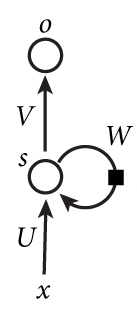
\includegraphics[scale=0.7]{rnn}
\caption{\textbf{RNN}}
\label{fig:rnn}
\end{figure}

\begin{figure}[h]
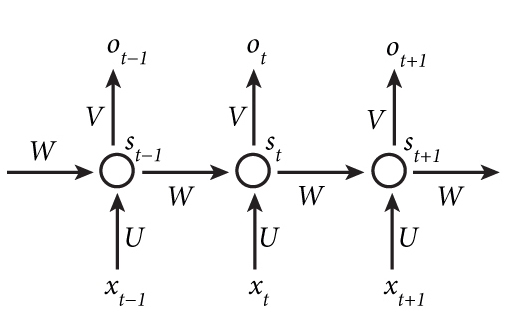
\includegraphics[scale=0.7]{rnn-unfold}
\caption{\textbf{RNN в развернутом виде}}
\label{fig:rnn-unfold}
\end{figure}

\noindent $U, W, V$~--- параметры RNN сети\\
$x_t$~--- вектор, соответствующий слову $t$ \\
$s_t$~--- информация о первых $t$ словах \\
$o_t$~--- выходной вектор

Хотя RNN является достаточно мощной моделью, у нее есть ряд недостатков, самый большой из которых~--- это так называемая <<проблема стирания градиента>>. Суть ее заключается в том, что RNN не может запоминать контекст в длинных последовательностях слов. Поэтому на смену RNN была изобретена LSTM (Long Short Term Memory) рекурсивная нейронная сеть, которая решает эту проблему[статья].

\begin{figure}[h]
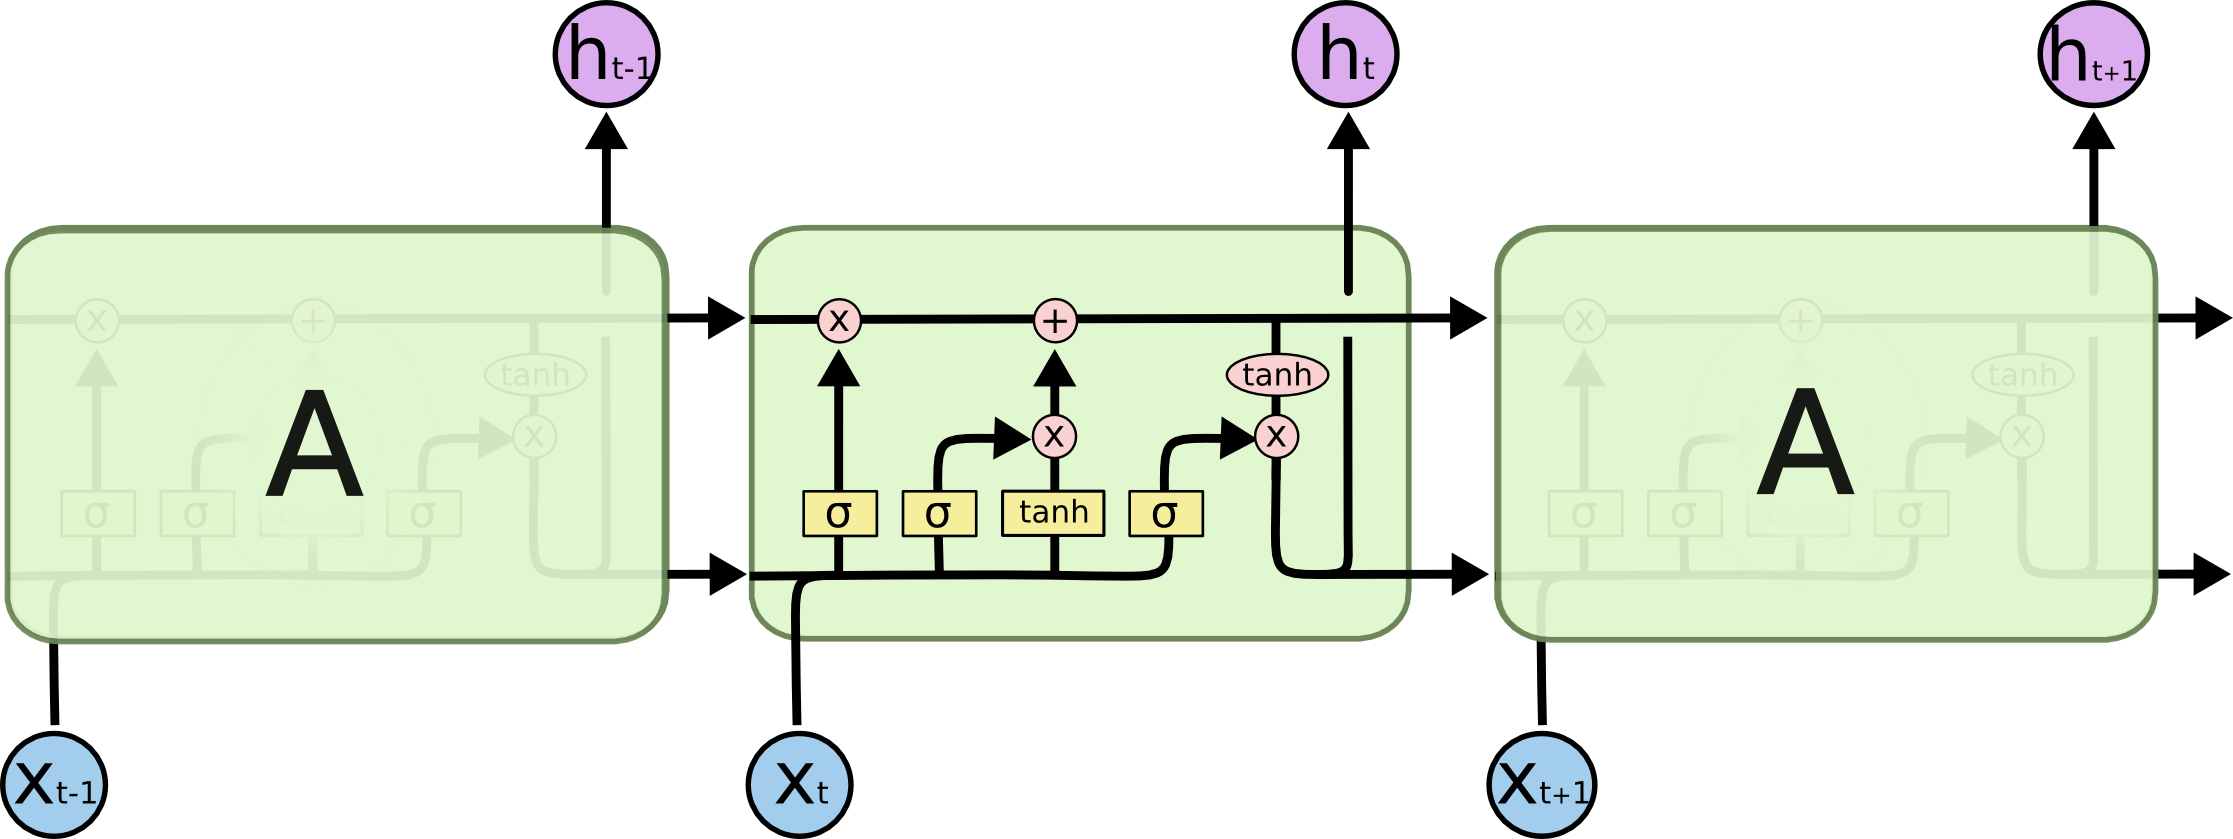
\includegraphics[scale=0.5]{lstm}
\caption{\textbf{LSTM}}
\label{fig:lstm}
\end{figure}

Таким образом, на вход LSTM подается предложение, и используется последний выходной вектор как векторное представление для задачи sentiment modelling [статья].

\subsection{CNN}
Convolutional Neural Network (CNN)~--- сверточные нейронные сети успешно показали себя в обработке и анализе изображений.[статья] Они работают подобно тому, как происходит распознавание образов в головной коре человека. Сверточные нейронные сети состоят из нескольких слоев, каждый из которых детектирует некоторые визуальные признаки изображения, такие как прямые линии, окружности. Признаки с предыдущего слоя используются для формирования более высокоуровневых визуальных признаков.

Преимуществом свойством сверточных нейронных сетей является выделение локалных пространственных признаков [статья]. В контексте изображений это означает, что визуальные признаки локализуются сначала на неболших квадратах, а далее объединяются в большие фигуры.

Оказывается, данный плюс можно использовать и в задаче sentiment modelling, если рассмотреть слова предложения как вектора некоторой размерности. Тогда если в предложении $n$ слов, 
и размерность векторного представления слова $d$, получаем матрицу $n \times d$, 
которую можно трактовать как изображение и применить к нему сверточную нейронную сеть.[статья].


\begin{figure}[h]
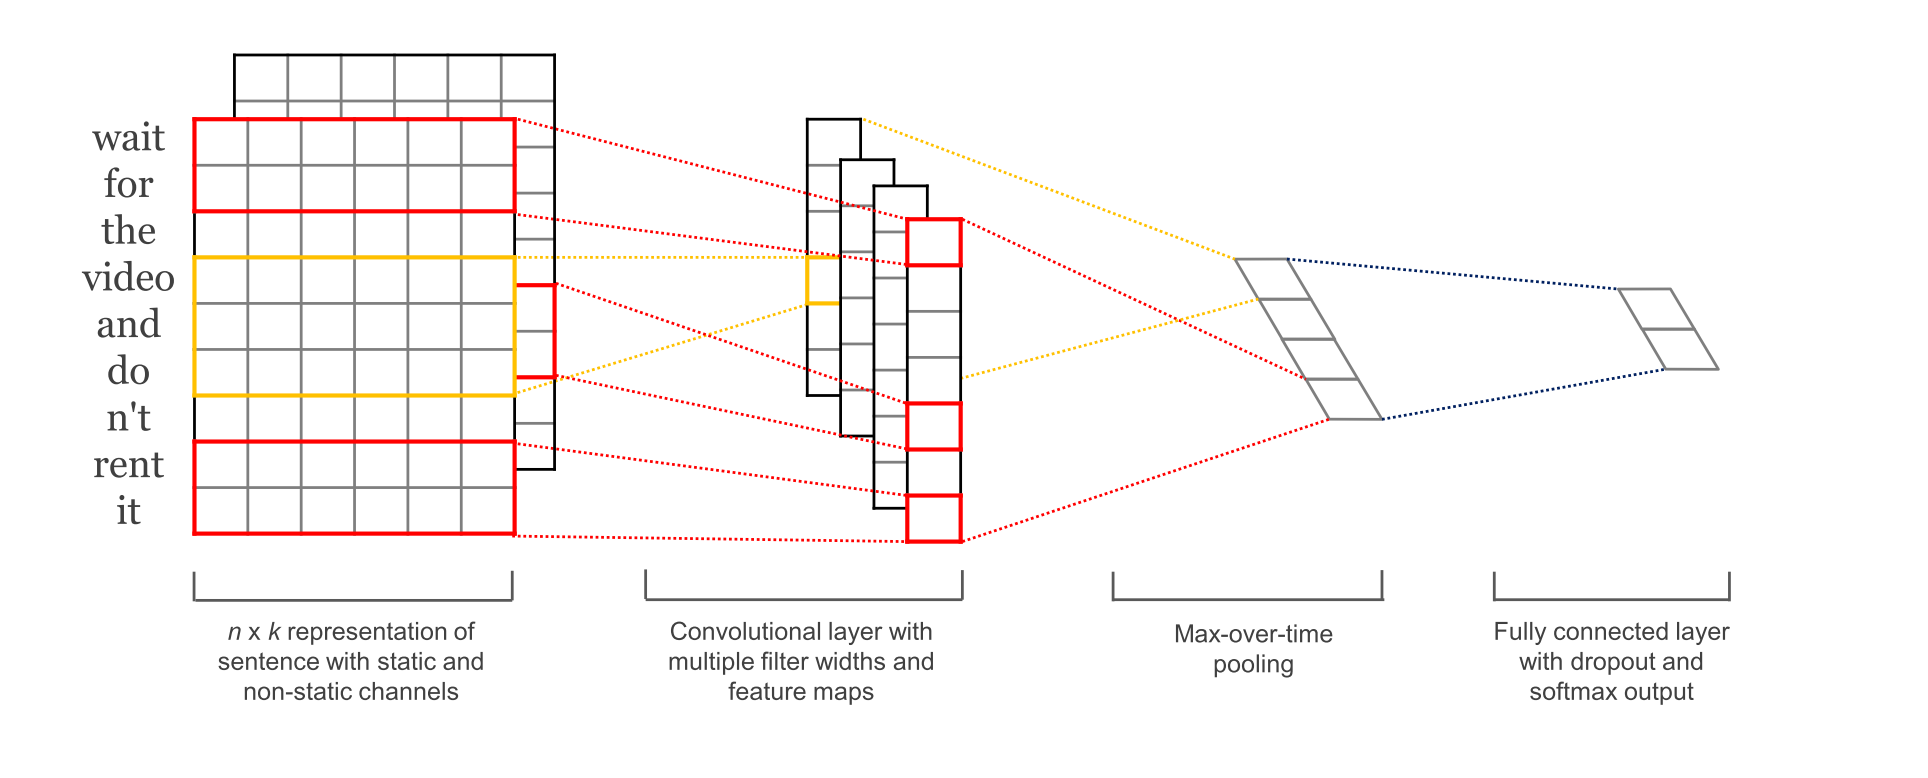
\includegraphics[scale=0.55]{cnn}
\caption{\textbf{CNN для предложения}}
\label{fig:cnn}
\end{figure}


\subsection{RNTN}
Еще одним важным подходом к решению задачи sentence modelling является использование 
дерева синтаксического разбора предложения. Вообще говоря, решения, исползующие этот подход, предполагают, что у предложения уже построено дерево синтаксического разбора. Построение дерева является отдельной достаточно важной задачей NLP. На данный момент существуют алгоритмы, которые делают это построение с очень хорошей точностью.[статья]. 
С другой стороны, обычно для таких решений не столь важно точное построение дерева, то есть они не критичны к неточностям в дереве разбора.

RNTN (Recursive Neural Tensor Network)~--- одно из решений, использующее дерево синтаксического разбора.
 